\begin{center}



\tikzset{every picture/.style={line width=0.75pt}} %set default line width to 0.75pt        

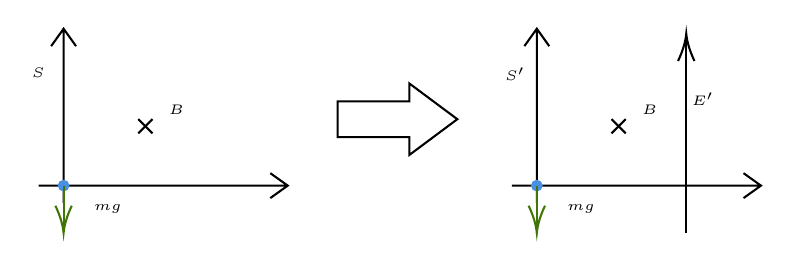
\begin{tikzpicture}[x=0.75pt,y=0.75pt,yscale=-1.2,xscale=1.2]
%uncomment if require: \path (0,300); %set diagram left start at 0, and has height of 300

%Straight Lines [id:da869864321489574] 
\draw    (210,94.3) -- (215.7,100) ;
%Straight Lines [id:da7393063880787207] 
\draw    (215.7,94.3) -- (210,100) ;

%Shape: Axis 2D [id:dp2610193597490549] 
\draw  (170,121) -- (270,121)(180,58) -- (180,128) (263,116) -- (270,121) -- (263,126) (175,65) -- (180,58) -- (185,65)  ;
%Shape: Circle [id:dp711598281784179] 
\draw  [color={rgb, 255:red, 74; green, 144; blue, 226 }  ,draw opacity=1 ][fill={rgb, 255:red, 74; green, 144; blue, 226 }  ,fill opacity=1 ] (178.09,121) .. controls (178.09,119.94) and (178.94,119.09) .. (180,119.09) .. controls (181.06,119.09) and (181.91,119.94) .. (181.91,121) .. controls (181.91,122.06) and (181.06,122.91) .. (180,122.91) .. controls (178.94,122.91) and (178.09,122.06) .. (178.09,121) -- cycle ;
%Straight Lines [id:da05120481576189717] 
\draw [color={rgb, 255:red, 65; green, 117; blue, 5 }  ,draw opacity=1 ]   (180,121) -- (180,138) ;
\draw [shift={(180,140)}, rotate = 270] [color={rgb, 255:red, 65; green, 117; blue, 5 }  ,draw opacity=1 ][line width=0.75]    (10.93,-3.29) .. controls (6.95,-1.4) and (3.31,-0.3) .. (0,0) .. controls (3.31,0.3) and (6.95,1.4) .. (10.93,3.29)   ;
%Straight Lines [id:da6674644989552678] 
\draw    (400,94.3) -- (405.7,100) ;
%Straight Lines [id:da20624873275002797] 
\draw    (405.7,94.3) -- (400,100) ;

%Shape: Axis 2D [id:dp8282527076559207] 
\draw  (360,121) -- (460,121)(370,58) -- (370,128) (453,116) -- (460,121) -- (453,126) (365,65) -- (370,58) -- (375,65)  ;
%Shape: Circle [id:dp6046113343970185] 
\draw  [color={rgb, 255:red, 74; green, 144; blue, 226 }  ,draw opacity=1 ][fill={rgb, 255:red, 74; green, 144; blue, 226 }  ,fill opacity=1 ] (368.09,121) .. controls (368.09,119.94) and (368.94,119.09) .. (370,119.09) .. controls (371.06,119.09) and (371.91,119.94) .. (371.91,121) .. controls (371.91,122.06) and (371.06,122.91) .. (370,122.91) .. controls (368.94,122.91) and (368.09,122.06) .. (368.09,121) -- cycle ;
%Straight Lines [id:da7526857324404845] 
\draw [color={rgb, 255:red, 65; green, 117; blue, 5 }  ,draw opacity=1 ]   (370,121) -- (370,138) ;
\draw [shift={(370,140)}, rotate = 270] [color={rgb, 255:red, 65; green, 117; blue, 5 }  ,draw opacity=1 ][line width=0.75]    (10.93,-3.29) .. controls (6.95,-1.4) and (3.31,-0.3) .. (0,0) .. controls (3.31,0.3) and (6.95,1.4) .. (10.93,3.29)   ;
%Right Arrow [id:dp6817029209016499] 
\draw   (290,87.17) -- (318.85,87.17) -- (318.85,80) -- (338.09,94.33) -- (318.85,108.67) -- (318.85,101.5) -- (290,101.5) -- cycle ;
%Straight Lines [id:da6241127557743624] 
\draw    (430,140) -- (430,62) ;
\draw [shift={(430,60)}, rotate = 90] [color={rgb, 255:red, 0; green, 0; blue, 0 }  ][line width=0.75]    (10.93,-3.29) .. controls (6.95,-1.4) and (3.31,-0.3) .. (0,0) .. controls (3.31,0.3) and (6.95,1.4) .. (10.93,3.29)   ;

% Text Node
\draw (221,87.4) node [anchor=north west][inner sep=0.75pt]  [font=\tiny]  {$B$};
% Text Node
\draw (191,127.4) node [anchor=north west][inner sep=0.75pt]  [font=\tiny]  {$mg$};
% Text Node
\draw (166,72.4) node [anchor=north west][inner sep=0.75pt]  [font=\tiny]  {$S$};
% Text Node
\draw (411,87.4) node [anchor=north west][inner sep=0.75pt]  [font=\tiny]  {$B$};
% Text Node
\draw (381,127.4) node [anchor=north west][inner sep=0.75pt]  [font=\tiny]  {$mg$};
% Text Node
\draw (356,72.4) node [anchor=north west][inner sep=0.75pt]  [font=\tiny]  {$S^{\prime }$};
% Text Node
\draw (431,82.4) node [anchor=north west][inner sep=0.75pt]  [font=\tiny]  {$E^{\prime }$};


\end{tikzpicture}


\end{center}